\documentclass{article}
\usepackage{amsmath}
\usepackage{amssymb}
\usepackage{mathrsfs}
\usepackage{physics}
\usepackage{comment}
\usepackage{mathtools}
\newcommand{\om}{\omega_n}
\newcommand{\adag}{a^\dagger}
\newcommand\Chi{\mathrm{X}}
\newtheorem{problem}{Problem}
\title{Extrapolation}
\author{Eesh Gupta}
\begin{document}
\maketitle
\tableofcontents
\newpage

Extrapolation is a technique in which we deliberately make noise rate worse in
order to get a more accurate result.
\section{Background}
\subsection{Richardson Extrapolation}
Suppose you have approximated \(A^\star\) as \(A(h)\) (assume \(h\) is
the error rate) but you want to make
a better approximation. Fortunately, you are also given a series

\begin{equation} \label{eq:1}
  A^\star = A(h) + a_0h^{k_0} + a_1h^{k_1} + a_2h^{k_2} + \ldots
\end{equation}
where \(a\)'s are unknown constants and \(k\)'s are known constants such that
\(h^{k_i} > h^{k_{i+1}}\). That is, the sequence on RHS of equation \ref{eq:1} is
decreasing. If we write the same equation in terms of Big Oh notation,
we have
\begin{equation} \label{eq:2}
  A^\star = A(h) + O(h^{k_0})
\end{equation}
The current error is on the order of \(O(h^{k_0})\).
Our need is to get a better approximation of \(A^\star\), let's say with
a higher order error \(O(h^{k_1})\) estimate. What do we do?
\begin{enumerate}
  \item \textit{Big Oh Notation} Rewrite the equation \ref{eq:1} as
  \begin{equation} \label{eq:3}
    A^\star = A(h) + a_0h^{k_0} + O(h^{k_1})
  \end{equation}
  In the following steps, our objective is to get rid of the term
   \(a_0h^{k_0}\) so we end up with an improved error bound of
   \(O(h^{k_1})\).
  \item \textit{Rescaling the Parameter} \(h\) as \(\frac{h}{t}\) where
  \(t\) is a constant (hopefully \(t \neq 1\)!).
  \begin{equation} \label{eq:4}
    A^\star = A(\frac{h}{t}) + a_0(\frac{h}{t})^{k_0} + O(h^{k_1})
  \end{equation}


  \item \textit{Ridding of a term from equation \ref{eq:1}:} Multiply equation \ref{eq:4} by
  \(t^{k_0}\), subtract equation \ref{eq:3} from the modified \ref{eq:4} and divide
  both sides of the resulting equation by \(t^{k_0} -1 \). Then we have
  \begin{equation} \label{eq:5}
    A^\star = \frac{t^{k_0}A(\frac{h}{t}) -A(h)}{t^{k_0} -1} + O(h^{k_1})
  \end{equation}
  We can repeat this process many times for different error rates to improve
  the aproximation further.
\end{enumerate}
\section{Extrapolating Noise via Rescaling Time}
\subsection{Series Expansion in Noise Parameter}
Our starting point is the following eqution
\begin{equation}
  \frac{\partial \rho}{\partial t} = -i[K(t), \rho] + \lambda\mathcal{L}(\rho)
\end{equation}
where the first term on RHS corresponds the time dependent qubit hamiltonian (set
of pauli gates acting on qubits with time dependent coupling coefficients) and the
second term accounts for noise. Here, \(\lambda\) is the streingth of noise, assumed
weak because of short depth circuits. While using a lindbladian superoperator may
imply that we are considering only markovian noise, we can also account for
non markovian noise by taking \(\mathcal{L}(\rho)\) as
\begin{equation}
  \lambda\mathcal{L}(\rho) = -i[V, \rho]
\end{equation}
where \(V\) is some hamiltonian.

Now, we can then remove the time evolution due
to qubit hamiltonian \(K(t)\) to zoom in on the noisy evolution in the
interation picture of \(K(t)\). This involves ``heisenburg-ing'' our noisy
superoperator \(\mathcal{L}\) and ``shrodinger-ing'' our density matrix
\(\rho\) with respect to \(K(t)\) to get the following partial differential equation:
\begin{equation}
  \frac{\partial}{\partial t}\rho_I(t) = + \lambda\mathcal{L}_{I, t}(\rho_I(t))
\end{equation}
From here on, we use some tricks relating to perturbative expansion and go back
to the schrodinger picture. After this process, we obtain the expectation value
of some observable A as
\begin{equation} \label{eq:10}
  E_K(\lambda) = E^\star + \sum_{k=1}^n a_k\lambda^k + R_{n+1}(\lambda, \mathcal{L}, T)
\end{equation}
Here, \(E_K(\lambda)\) is the expectation value of \(A\) given noise rate of
\(\lambda\), \(E^*\) is the noiseless expectation value of \(A\), \(a_k\) hides huge integrals
involving the noisy superoperator \(\mathcal{L}\), \(R\) is the ``remainder''
of the infinite series and \(T\) is the time for which noisy evolution lasts.

Fortunately, \(R\) is bounded so the series is decreasing. Hence, we can apply
richarson extrapolati to improve upon our approximation of noiseless
expectation value \(E^\star\).
\subsection{Experimental Rescaling of the noise parameter}
The chief concern in this section is how to control the noise
parameters \(\lambda\) in an experimental setting. One possible solution
is to rescale the time \(T\) for which the noisy evolution lasts. This
may result in us either ``waiting longer'' to measure the results, ``slowing down''
the gate operations or a combination of both. Using some clever substitution techniques inside integrals,
we can show that rescaling time \(T\) results in a rescaled noise rate
 \(\lambda\).

 Note that in this case, noise is assumed constant in time. This is not always true. For example,
 consider the figure below:
\begin{figure}[!htb]
	\centering
	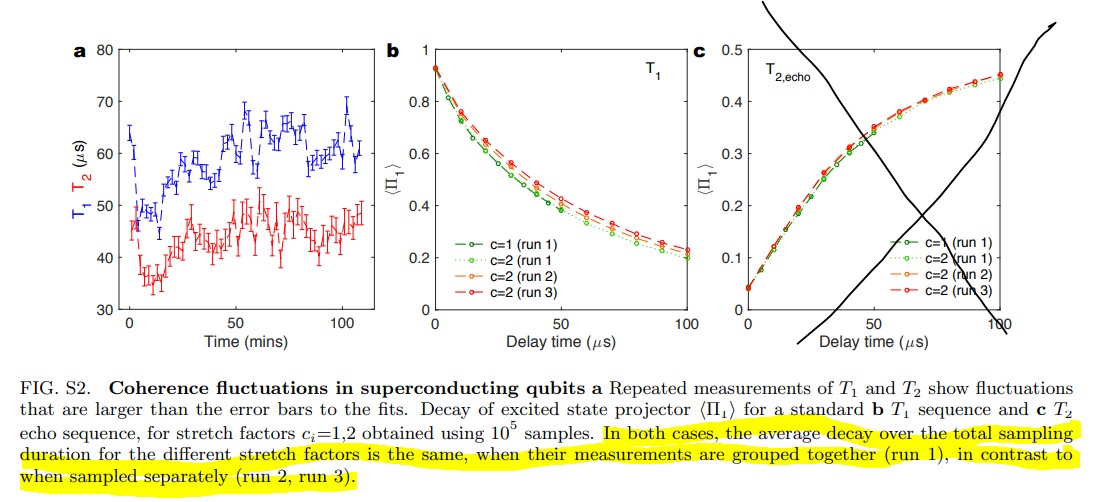
\includegraphics[width=1.4\textwidth]{img/main-f791e832.png}
	\caption{Figure from https://arxiv.org/pdf/1805.04492.pdf}
	\label{fig1}
\end{figure}

Figure \ref{fig1} shows decoherence times \(T_1, T_2\) on a 5 qubit superconducting
processor at IBM. \(T_1\) is a decay constant which measures how long it takes for a qubit
in excited state \(\ket{1}\) to relax to state \(\ket{0}\). On the other hand, \(T_2\)
measures the time it takes for a qubit in state \(\ket{+} = \frac{\ket{0}+ \ket{1}}{2}\) to turn into mixture of \(\ket{+}\) and \(\ket{-}\). Simply put,
\(T_1\) is the relaxation time constant and \(T_2\) is the dephasing time constant.

In \ref{fig1} a, we see how the decoherence times fluctuate over 2 hours. These
fluctuations shows that the noise rate is not constant in time. Futher \ref{fig1} b
(which I do not understand completely) tells us that we need to perform ``rescaled''
experiments shortly after one another. If we wait too long between experiments,
our results would be affected and extrapolated results would be less accurate.


\subsection{Error bounds on the noise free parameter}
Once we can rescale our noise rate \(\lambda\), we are ready to perform
Richardson Extrapolation. In our earlier discussion on this trick, we rescaled
our noise just once to improve our error bound from \(O(h^{k_0})\) to \(O(h^{k_1})\).
However, in general, we can perform multiple rescalings and improve our
error bounds by multiple orders with only a few equations. So in this scenario,
we will scale our noise rate \(n\) times and hence cancel \(n\) terms from
RHS of equation \(\ref{eq:10}\). To do so, we need to combine
expectation values with distinct noise rates as
\begin{equation}
  E^n_{K}(\lambda) = \sum^n_{j=0} \gamma_j \hat{E}_K(c_j \lambda)
\end{equation}
where \(\gamma_j\) is the weight of the expectation value with noise rate
scaled as \(c_j \lambda\). To do \(n\) steps at once, we have to abide by 2
constraints:
\begin{enumerate}
  \item \(E^\star\) has to end up normalized at the end. So
  \[\sum_{j=0}^n \gamma_j= 1\]
  \item We need to cancel out \(n\) terms from RHS of equation \(\ref{eq:10}\)
   to improve our aprroximation. So
   \[\sum_{j=0}^n \gamma_j c^k_j= 0 \text{  for  } k = 1 \ldots n\]
\end{enumerate}
(\(***\) It's not clear how such constraints result in the equations presented in the above text. But I am just writing out the function of those equations without showing all the math. That can be found however in equation 36 of the Temme paper)


This results in
\[E^\star = E^n_{K}(\lambda) + O(\lambda^{n+1}) \]
Note that strecth factor \(c_j >1\) for \(j = 1, \ldots, n\) i.e. we are scaling up the noise rate. In the numerical literature, it is common to scale down the noise rate. However, the result is just the same so this point is not so important.

\section{Extrapolating Noise via Pauli Gates}
\subsection{Stochastic vs Non stochastic noise}
In the pauli error model, errors are \textit{stochastic} if the noise superoperator \(\mathcal{N}\) can be written in the form
\begin{equation} \label{eq101}
\mathcal{N} = (1-\epsilon)\mathcal{I} + \epsilon\mathcal{E}
\end{equation}
where \(\mathcal{I}\) is the identity operation and \(\mathcal{E}\) is some
error that occurs with probabilty \(\epsilon\). Note that \(\mathcal{E}\) is a
valid quantum operation i.e. it is TPCP (Trace-preserving-completely-positive)
map.

Then, stochastic or ``probabilitic'' error models are those in which the system remains unchanged
with some probability \(1-\epsilon\) and system changes due to error with
probability \(\epsilon\). Then what does \textit{non-stochastic} error mean?
A non-stochastic error is simply one which cannot be expressed in such a form as
\ref{eq101}. They are also known as coherent noise.
\subsection{Reformulating Extrapolation}

\subsection{Pauli Twirling}
\subsection{Noise Amplification}
Let \(\epsilion_{i,j}\) be the the 2 qubit error rate between qubits \(q_i\)
and \(q_j\). Because of Pauli Twirling, there exists another interpretation
of \(\epsilion_{i,j}\): the probability of randomly applying 2 qubit pauli
gates on qubits \(q_i, q_j\). Then to increase this error rate by some factor
let's say \(r\), we would need to apply 2 pauli operations \(\sigma_c^{e},
\sigma_t^{f}\) randomly with probability \((r-1)\epsilion_{i,j}\). Why so?
Because this gives us a new error rate of \(\epsilion_new = \epsilion_{i,j}
+ (r-1)\epsilion_{i,j}\). Here, the first term on RHS is due to the error rate
of the controlled phase gate (or the CNOT gate). And the second term on RHS is
due to the additional pauli gates \(\sigma_c^{e},
\sigma_t^{f}\).
\end{document}
